\documentclass[tikz,border=8pt]{standalone}
\usepackage{amsmath}
\usetikzlibrary{arrows.meta,positioning}

\begin{document}
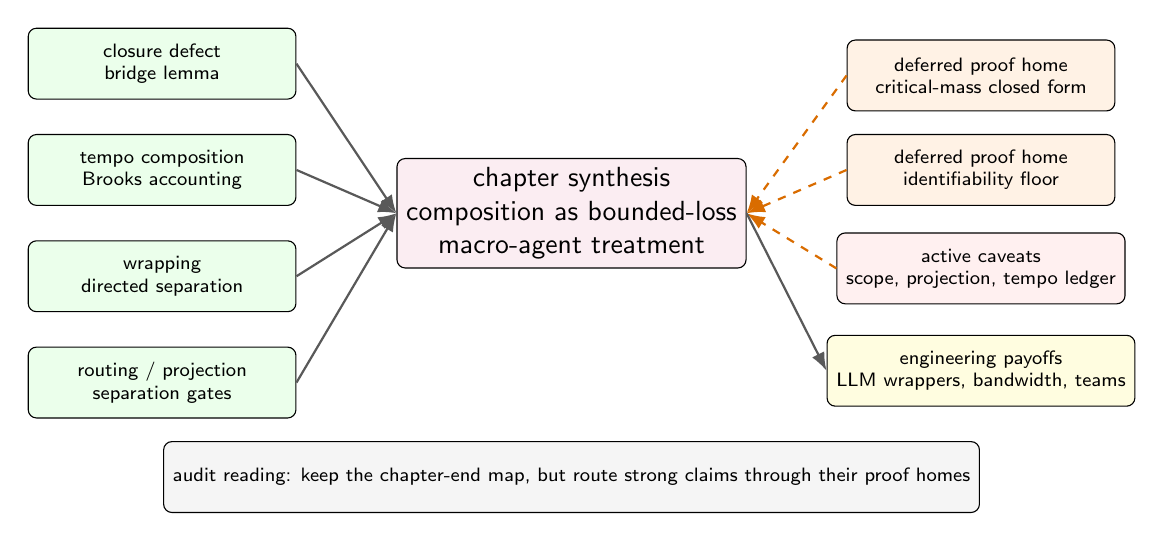
\begin{tikzpicture}[
  font=\sffamily,
  box/.style={draw, rounded corners=3pt, align=center, minimum width=39mm, minimum height=11mm, fill=white},
  small/.style={draw, rounded corners=3pt, align=center, font=\sffamily\scriptsize, minimum width=34mm, minimum height=9mm, fill=white},
  arrow/.style={-Latex, thick, draw=black!65},
  warn/.style={-Latex, thick, dashed, draw=orange!85!black}
]

\node[box, fill=purple!7] (hub) at (0,0)
  {chapter synthesis\\composition as bounded-loss\\macro-agent treatment};

\node[small, fill=green!8] (closure) at (-5.2,1.9)
  {closure defect\\bridge lemma};
\node[small, fill=green!8] (tempo) at (-5.2,0.55)
  {tempo composition\\Brooks accounting};
\node[small, fill=green!8] (wrap) at (-5.2,-0.8)
  {wrapping\\directed separation};
\node[small, fill=green!8] (ds) at (-5.2,-2.15)
  {routing / projection\\separation gates};

\draw[arrow] (closure.east) -- (hub.west);
\draw[arrow] (tempo.east) -- (hub.west);
\draw[arrow] (wrap.east) -- (hub.west);
\draw[arrow] (ds.east) -- (hub.west);

\node[small, fill=orange!10] (crit) at (5.2,1.75)
  {deferred proof home\\critical-mass closed form};
\node[small, fill=orange!10] (floor) at (5.2,0.55)
  {deferred proof home\\identifiability floor};
\node[small, fill=red!6] (caveat) at (5.2,-0.7)
  {active caveats\\scope, projection, tempo ledger};
\node[small, fill=yellow!12] (payoff) at (5.2,-2.0)
  {engineering payoffs\\LLM wrappers, bandwidth, teams};

\draw[warn] (crit.west) -- (hub.east);
\draw[warn] (floor.west) -- (hub.east);
\draw[warn] (caveat.west) -- (hub.east);
\draw[arrow] (hub.east) -- (payoff.west);

\node[small, fill=gray!8, minimum width=76mm] at (0,-3.35)
  {audit reading: keep the chapter-end map, but route strong claims through their proof homes};

\end{tikzpicture}
\end{document}
